\section{TT\&C}
\f{terminology}
\begin{itemize}
 \item radiocommunication service RR20 -- involving the transmission/reception of radio waves
 \item frequency allocation RR17 -- entry in the table of frequencies of given band for radiocommunication services
 \item frequency assignment RR18 -- authorisation to use radio frequency under conditions
\end{itemize}

\f{communication delay}
\begin{figure}[ht!]
 \centering
 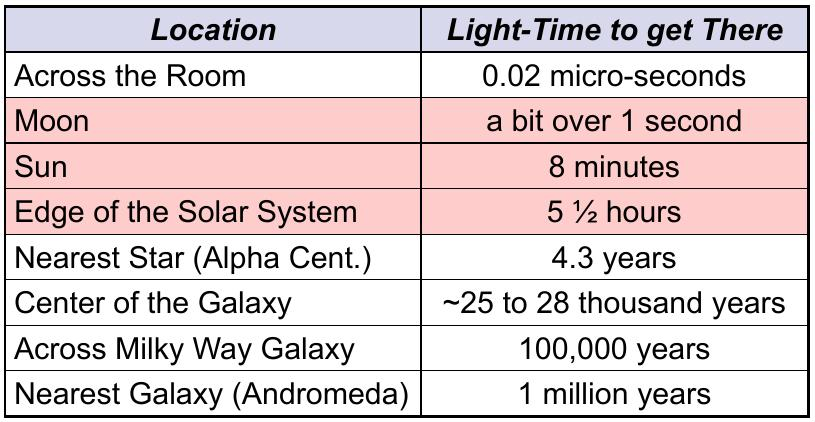
\includegraphics[scale=0.6]{commdelay}
\end{figure}

\f{bands -- frequencies \& wavelength}
\begin{figure}[ht!]
 \centering
 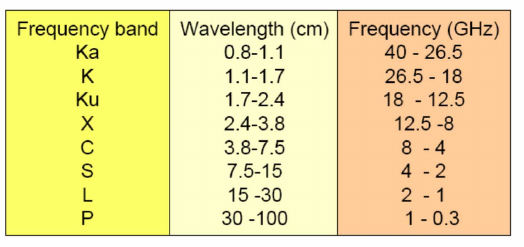
\includegraphics[scale=0.6]{bands}
\end{figure}

\f{band usage}
\begin{itemize}
 \item S: SOHO, XMM-Newton, Cluster, Integral
 \item X: Mars Express, Rosetta, Venus Express, Herschel, Plank
 \item $K_a$: LISA Pathfinder, Gaia, James Webb Space Telescope, BepiColumbo
\end{itemize}

\f{transponder operations}
\begin{itemize}
 \item Uplink Carrier, Carrier + Telecommand, Carrier + TC + Ranging
 \item Downlink Carrier, Carrier + Telemetry, Carrier + TM + Ranging
 \item auto-switch into coherent mode
\end{itemize}

\f{reasons for modulation}
\begin{itemize}
 \item to separate signals
 \item to select correct frequency
 \item easier transmission
\end{itemize}

\f{typical modulation types}
\begin{itemize}
 \item uplink: $2 \frac{kbits}{s}$ bitstream is phase-modulated onto 16kHz carrier
 \item downlink: bi-phase stream directly phase-modulated onto carrier, residual carrier recovered at groundstation before demodulation
\end{itemize}

\f{Link-Design Key Parameters}
\begin{itemize}
 \item Antenna Directivity and Gain
 \item Antenna Effective Area
 \item Dish Antenna Gain
 \item Free-Space Path Loss
 \item Effective Isotropic Radiated Power (EIRP) -- product of transmit power and transmit antenna gain
 \item Thermal Noise -- voltage fluctuations by moving charge carriers in conducting medium
 \item Figure-of-Merit (G/T) -- capability to recieve signal
\end{itemize}

\f{Directivity and gain}
\begin{itemize}
 \item all Antennas are stronger in one direction
 \item inverse square law of electromagnetic radiation $\frac{1}{r^2}$
 \item effective area of antenna is proportional to gain
 \item gain-beamwidth tradeoff: narrower beam$\leftrightarrow$more gain, less coverage $\rightarrow$ more stringent positioning of SC
 \item beamwidth inversly proportional to antenna size
 \item free-space path loss: doubling frequency implies 6 dB increase in path loss
\end{itemize}

\f{basic link design}
\begin{figure}[ht!]
 \centering
 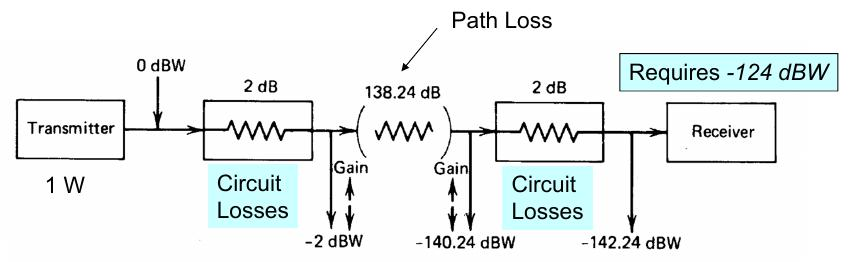
\includegraphics[scale=0.6]{linkdesign}
\end{figure}

\f{synchronisation}
\begin{itemize}
 \item signal influenced by: frequency offset, phase offset, hardware delays
 \item recievers try to:
 \begin{itemize}
  \item detach information from carrier (frequency)
  \item estimate and remove offsets
 \end{itemize}
 \item demodulation and estimation
 \item phase lock loop techniques
 \item Typical Bandwidth: 800 Hz (near-Earth), or 20 Hz (Deep-Space)
\end{itemize}

\f{system- \& error budgets}
\begin{itemize}
 \item predicting and managing variability
 \item propagete errors through a system
 \item link aspects of design and environment to capabilities and tolerances
 \item determine and track critical parameters
\end{itemize}

\f{channel encoding}
\begin{itemize}
 \item encoder takes $k$ incoming bits, maps them to $n$ outgoing bits ($n> k$)
 \item $n-k$ bits for error detection
 \item decoder does reverse process
\end{itemize}